%%%%%%%%%%Packages%%%%%%%%%

\documentclass[11pt, titlepage, letterpaper, twoside]{article}
\usepackage{amsmath, amsthm, amssymb}
\usepackage{hyperref, pgf, tikz}
\usepackage{fancyhdr}
\usetikzlibrary{arrows}
\usepackage[margin=1.25in]{geometry}

%%%%%%%%%%%%%%%%%%%%%%%%%%%

%%%%%%%%%%New Commands%%%%%%%%%



%%%%%%%%%%%%%%%%%%%%%%%%%%%
\pagestyle{fancy}
\frenchspacing

\lhead{Lab \#7 }  %insert lab # here
\rhead{\thepage}
\cfoot{}

\title{\textbf{Refraction and Standing Waves} \\ \ \\ \large Lab \#7 }
\author{Name: Aidan Fitzgerald \\ Partners: Julia Hou, Ariella Kahan, Jongyoul Lee, Kelly Luo, Vyshnavi Parthipan, Jeffrey Zou}
\date{June 13, 2016}
\begin{document}

\maketitle

\begin{center}
\LARGE Refraction and Standing Waves
\end{center}

\section*{Objective}

Measure the wavelength of a microwave by creating a standing wave and calculate the index of refraction of a material
using Snell's law.

\section{Introduction}

\subsection{Standing waves}

A standing wave is a wave whose energy density at every point remains constant, or a wave that does not propagate.
The points at which the energy density is zero are called the nodes of the wave, and the points where the energy
density is a maximum are called the antinodes.

A standing wave is generated by resonance when a traveling plane wave of wavelength $\lambda$ reflects back on itself
from a wall that is some integer multiple of $\lambda/2$ away from the source and interferes with itself. The horns
of the microwave receiver reflect some radiation, so the transmitter and receiver can be placed facing each other at
a distance $n\lambda/2$ apart (for any natural number $n$) to create a standing wave. When this happens, the intensity
reading will be at a maximum.

\subsection{Refraction}

An electromagnetic wave is refracted, or bent, when it passes from one medium to another medium with a different index
of refraction. Snell's law, named after Dutch astronomer Willebrord Snellius, relates the indices of refraction of the
materials the light passes through and the angles at which it enters and leaves the boundary. If $\theta_1$ is the
angle between the direction of the light before crossing and the surface normal of the boundary, $\theta_2$ is the
angle between the direction after crossing and the surface normal, and $n_1$ are the indices of refraction of the first
and second materials the light passes through, then

\begin{equation}
  n_1 \sin \theta_1 = n_2 \sin \theta_2.
\end{equation}

The index of refraction of air is approximately 1.

\section{Procedures and Results}

\subsection{Standing waves}

We set up the microwave system so that the transmitter and receiver diodes were approximately 70 cm and then slid them
a few centimeters farther apart to get a maximum intensity reading. Then, we slid them farther apart, counting the
times that the intensity reading hit a local minimum, stopping at a local maximum. We recorded the initial and final
positions of the units and the number of minima passed.

\begin{table}[h!]
\centering
\caption{Standing wave measurements}
\label{stwav}
\begin{tabular}{|l|l|l|}
\hline
Initial position ($r_i$) & Number of minima passed ($n$) & Final position ($r_f$) \\ \hline
74.9 cm                  & 10                            & 90 cm                  \\ \hline
73.3 cm                  & 11                            & 88.3 cm                \\ \hline
\end{tabular}
\end{table}

\subsection{Refraction}

We set up the microwave system with a right triangular ethafoam (polyethylene foam) prism mold on the center of the goniometer, then
filled the prism mold with polystyrene pellets. We aligned the prism mold so that its longer leg was facing perpendicular to the
transmitter arm of the goniometer, then turned the transmitter on. Next, we moved the receiver arm until the intensity reading was
a maximum and recorded the angle $\varphi$ between the refracted ray and the incident ray.

Because the prism mold is a right triangle, the angle of incidence $\theta_1$ is equal to the angle adjacent to the leg facing
the transmitter. We measured this angle using a protractor. The angle of refraction $\theta_2 = \theta_1 + \varphi$.

\begin{figure}[h!]
  \centering
  \caption{Refraction setup}
  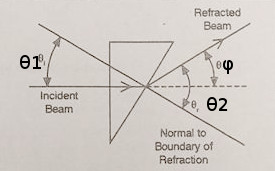
\includegraphics{refraction}
\end{figure}

\begin{align*}
  \theta_1 &= 48^\circ \\
  \varphi  &= 12^\circ \\
  \theta_2 &= \theta_1 + \varphi = 60^\circ
\end{align*}

\pagebreak

\section{Discussion}

\subsection{Standing waves}

Using the data in Table \ref{stwav}, we can calculate the wavelength $\lambda$. A sample calculation is shown for the first entry:

\begin{align*}
  n\lambda / 2  &= r_f - r_i \\
  10\lambda / 2 &= 90\,\mathrm{cm} - 74.9\,\mathrm{cm} \\
  5\lambda      &= 15.1\,\mathrm{cm} \\
  \lambda       &= 3.02\,\mathrm{cm}
\end{align*}

Using the second row of data we obtain $\lambda = 2.73\,\mathrm{cm}$.

The percent difference between these two values is approximately 10\%.

\subsection{Refraction}

When light enters a right triangular prism through a leg of the triangle, it is not refracted because it enters perpendicular
to the surface. However, when it leaves the prism, it is refracted according to Snell's law.

\begin{align*}
  n_1 \sin \theta_1 &= n_2 \sin \theta_2 \\
  n_1 \sin 48^\circ &= 1.0 \sin 60^\circ \\
  n_1 &= 1.0 \,\frac{\sin 60^\circ}{\sin 48^\circ} \\
  n_1 &\approx 1.17
\end{align*}

The index of refraction of the prism mold is $n_1 \approx 1.17$.

\section{Conclusion}

We can use the properties of standing waves to determine the wavelength of a wave, and we can use Snell's law to find the
index of refraction of a material.

\end{document}
